\section{DESARROLLO} 

\subsection{Analisis}
\begin{itemize}
	\item Casos de Uso
	\begin{figure}[H]
		\begin{center}
			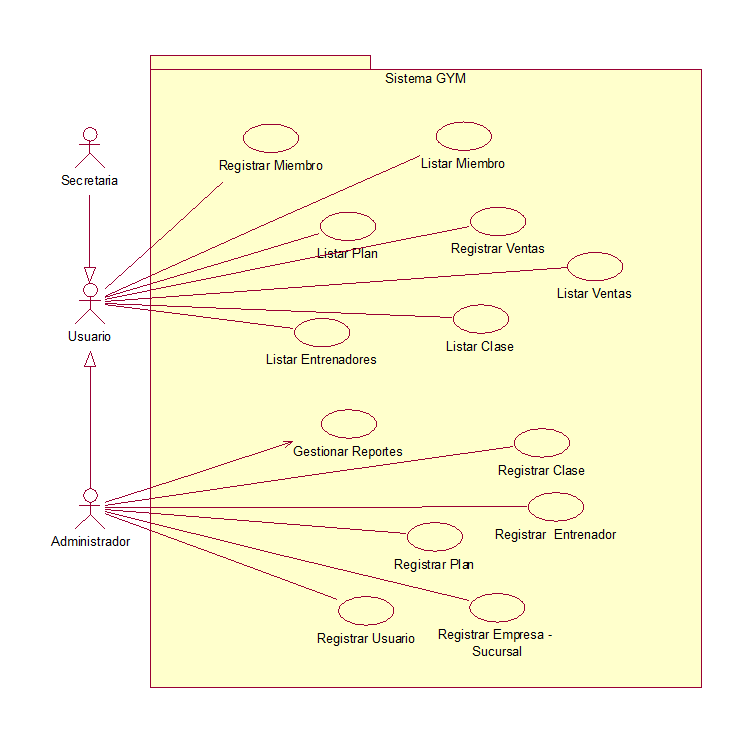
\includegraphics[width=15cm]{./Imagenes/CasosDeUso}
		\end{center}
	\end{figure}
\end{itemize}


\subsection{Diseño}
\begin{itemize}
	\item Diagrama de Clases
\begin{center}
	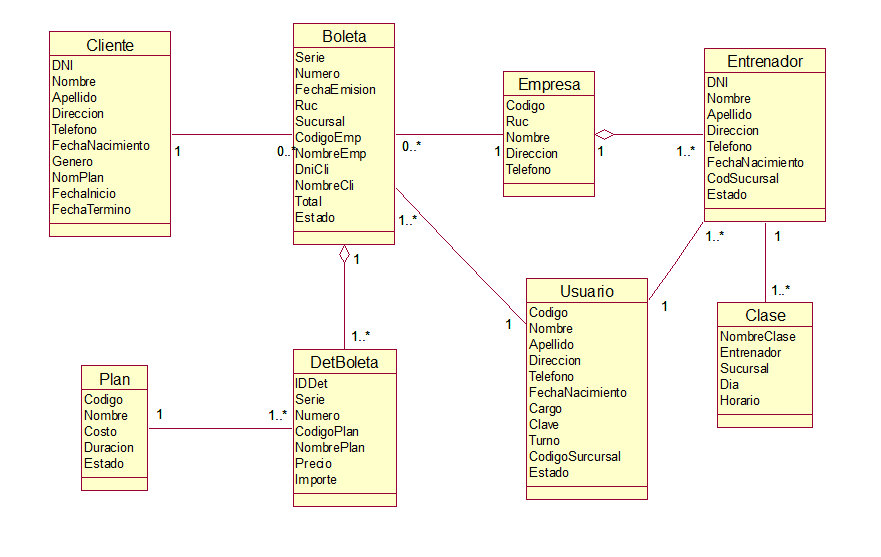
\includegraphics[width=15cm]{./Imagenes/DiagramaClases}
\end{center}
	\item Modelo Entidad Relación
\begin{figure}[H]
		\begin{center}
			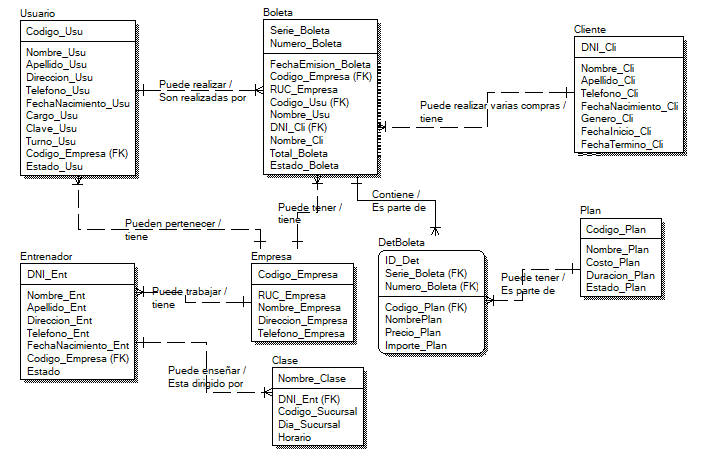
\includegraphics[width=17cm]{./Imagenes/EntidadRelacion}
		\end{center}
	\end{figure}
\end{itemize}



\subsection{Pruebas}
Las pruebas realizadas fueron las siguientes:
\begin{itemize}
	\item ObtenerAlEntrenadorPorCodigo 
\begin{center}
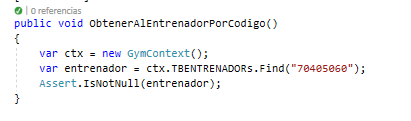
\includegraphics[width=15cm]{./Imagenes/prueba1.png}
\end{center}
Sentencia SQL generada:
\begin{center}
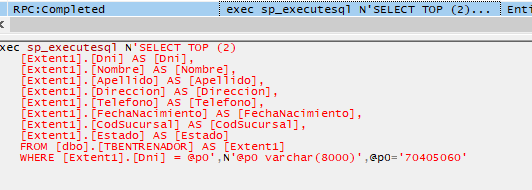
\includegraphics[width=15cm]{./Imagenes/profile1.png}
\end{center}
	\item AgregarDosPlanesdeGimnasio
\begin{center}
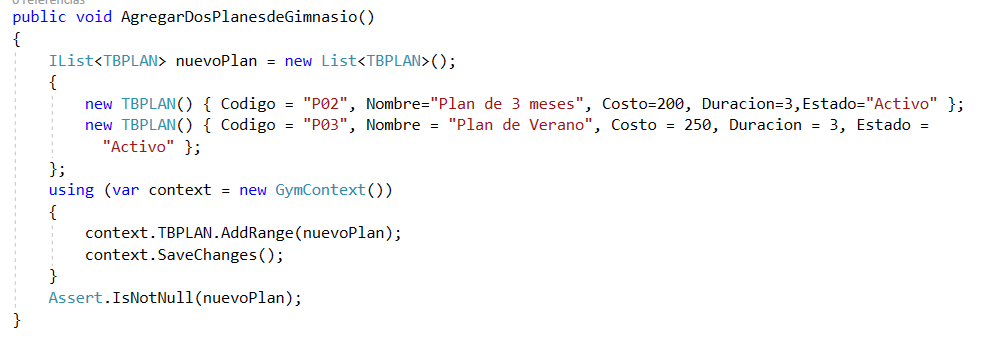
\includegraphics[width=17cm]{./Imagenes/prueba2.png}
\end{center}
Sentencia SQL generada:
\begin{center}
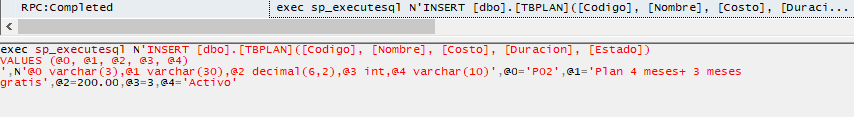
\includegraphics[width=17cm, height=3cm]{./Imagenes/profile2-1.png}
\end{center}
\begin{center}
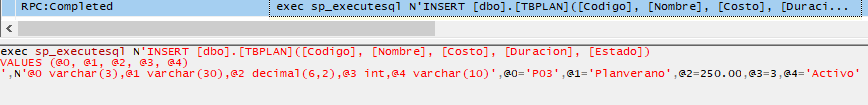
\includegraphics[width=17cm, height=3cm]{./Imagenes/profile2-2.png}
\end{center}
	\item ObtenerListaDeClasesPorNombreAscendiente
\begin{center}
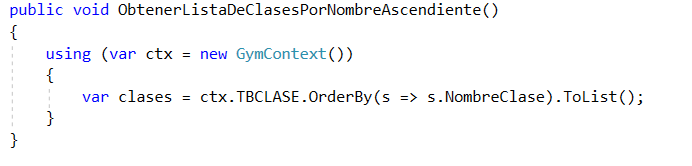
\includegraphics[width=15cm]{./Imagenes/prueba3.png}
\end{center}
Sentencia SQL generada:
\begin{center}
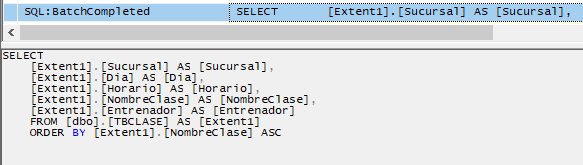
\includegraphics[width=15cm]{./Imagenes/profile3.png}
\end{center}
	\item BuscarTodaslasBoletasPorEmpleado
\begin{center}
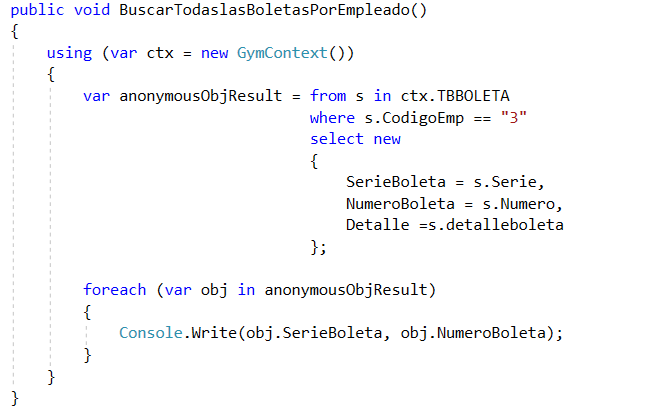
\includegraphics[width=15cm]{./Imagenes/prueba4.png}
\end{center}
Sentencia SQL generada:
\begin{center}
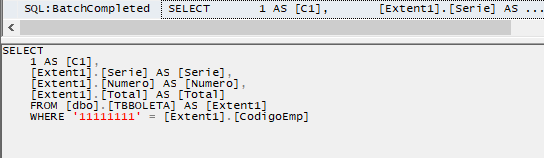
\includegraphics[width=15cm]{./Imagenes/profile4.png}
\end{center}
	\item EliminarUnPlanDeGimnasioPorCodigo
\begin{center}
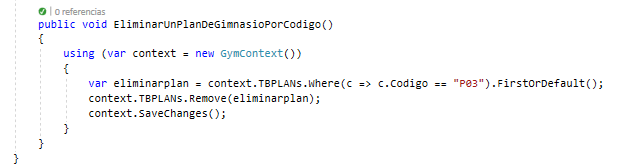
\includegraphics[width=15cm]{./Imagenes/prueba5.png}
\end{center}
Sentencia SQL generada:
\begin{center}
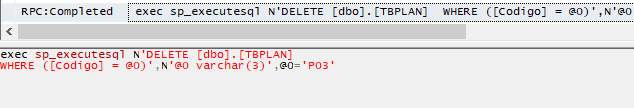
\includegraphics[width=15cm]{./Imagenes/profile5.png}
\end{center}
\end{itemize}
\subsection{API/Postman}

             \begin{center}
			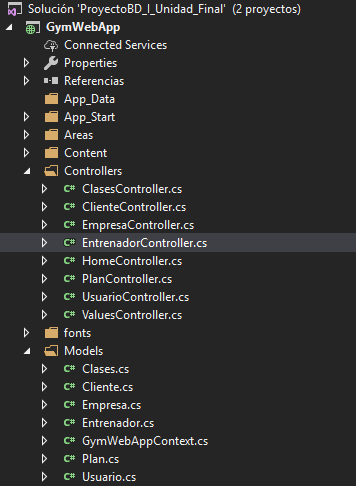
\includegraphics[width=10cm]{./Imagenes/1}
             \end{center}
\begin{itemize}
\item Del controlador Cliente, hacemos clic en POST Cliente para agregar un registro.
    \begin{center}
			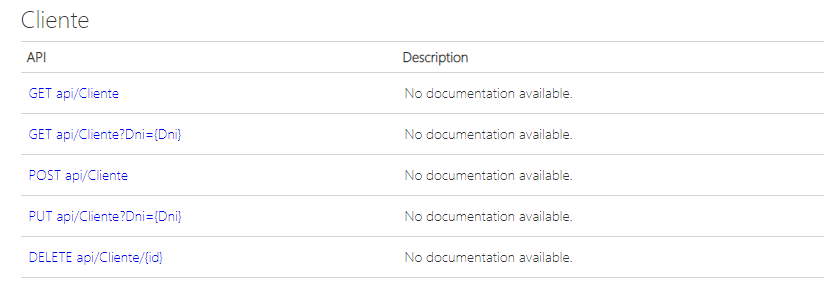
\includegraphics[width=16cm]{./Imagenes/cl}
             \end{center}
Copiamos el formato de la cadena, y luego la pegamos en Postman, donde agregaremos un nuevo cliente.
    \begin{center}
			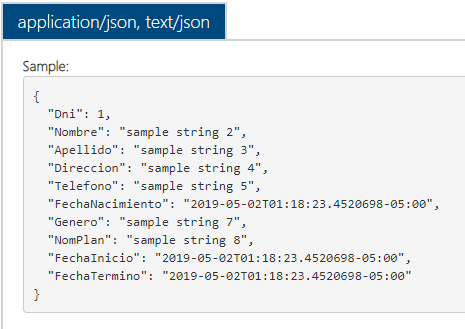
\includegraphics[width=10cm]{./Imagenes/clp}
             \end{center}
 \begin{center}
			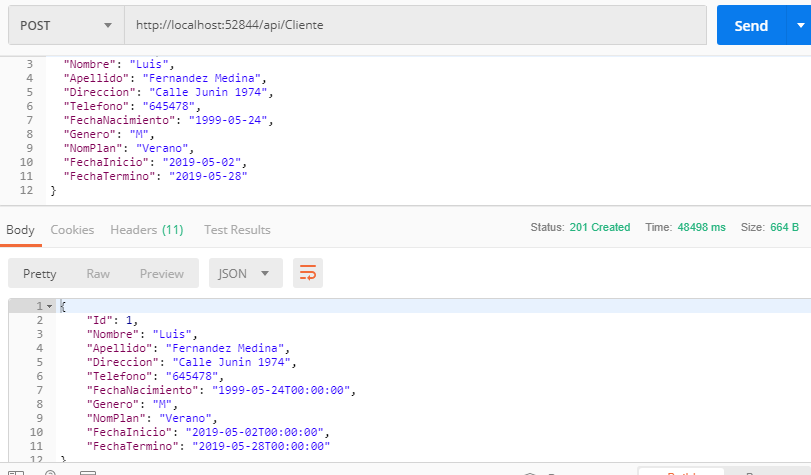
\includegraphics[width=15cm]{./Imagenes/pcl}
             \end{center}
\item Comprobamos que ha sido agregado el nuevo registro en la tabla con GET.
 \begin{center}
			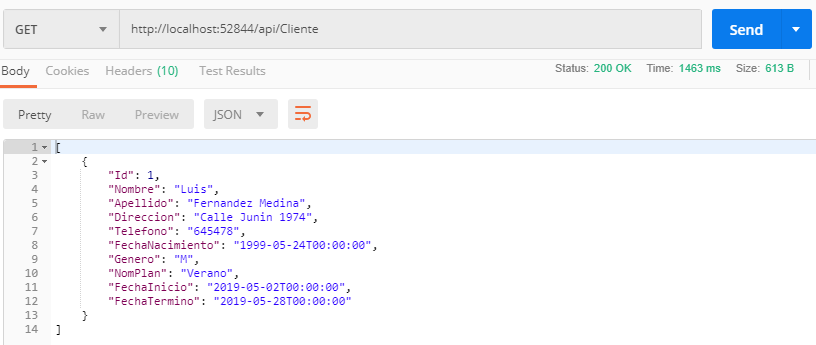
\includegraphics[width=15cm]{./Imagenes/gcl}
             \end{center}
\item Del controlador Usuario, hacemos clic en POST Usuario para agregar un registro.
 \begin{center}
			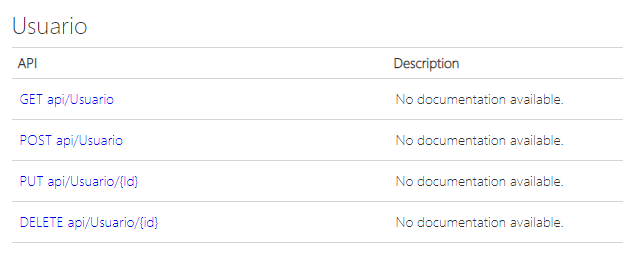
\includegraphics[width=14cm]{./Imagenes/us}
             \end{center}
Copiamos el formato de la cadena, y luego la pegamos en Postman, donde agregaremos un nuevo usuario.
 \begin{center}
			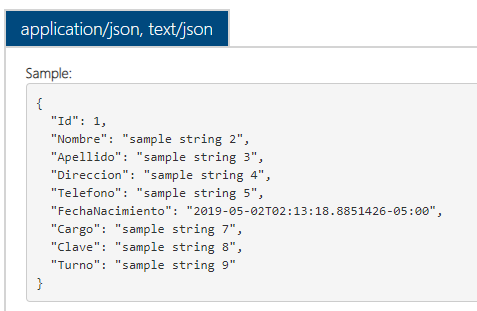
\includegraphics[width=10cm]{./Imagenes/pusu}
             \end{center}
 \begin{center}
			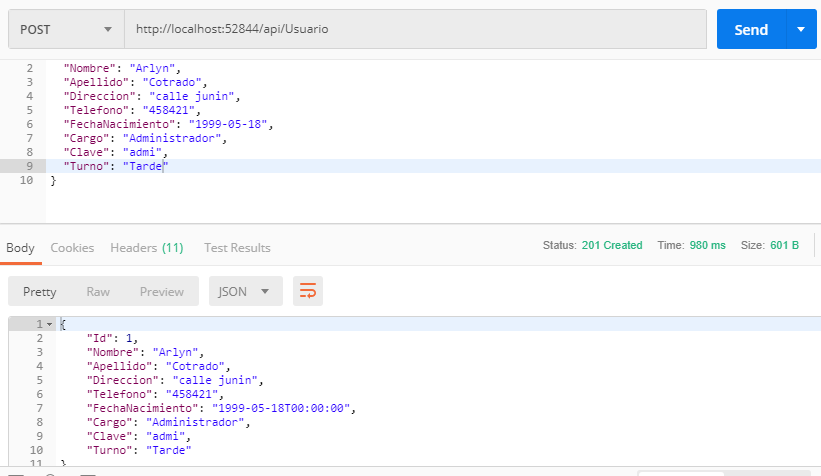
\includegraphics[width=15cm]{./Imagenes/usu}
             \end{center}
\item Del controlador Entrenador, hacemos clic en POST Entrenador para agregar un registro.
 \begin{center}
			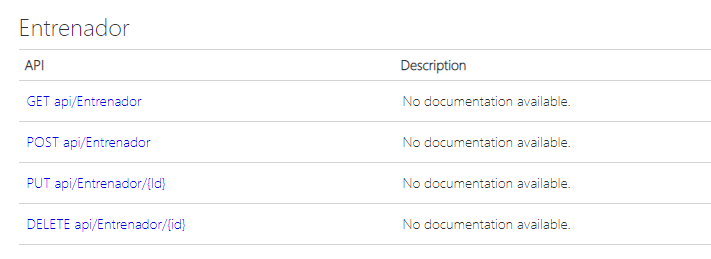
\includegraphics[width=15cm]{./Imagenes/ent}
             \end{center}
Copiamos el formato de la cadena, y luego la pegamos en Postman, donde agregaremos un nuevo entrenador.
 \begin{center}
			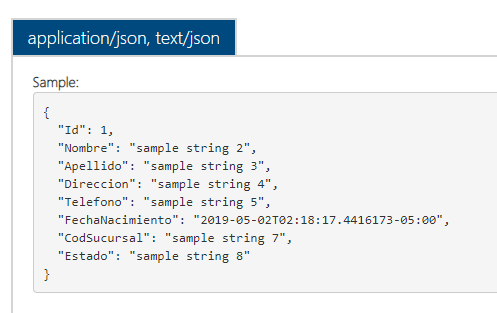
\includegraphics[width=10cm]{./Imagenes/e}
             \end{center}
 \begin{center}
			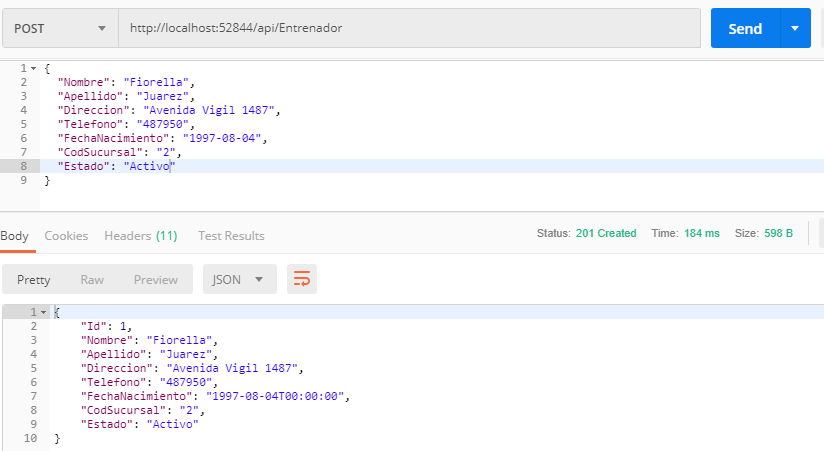
\includegraphics[width=15cm]{./Imagenes/pent}
             \end{center}
\item Del controlador Plan, hacemos clic en POST Plan para agregar un registro.
 \begin{center}
			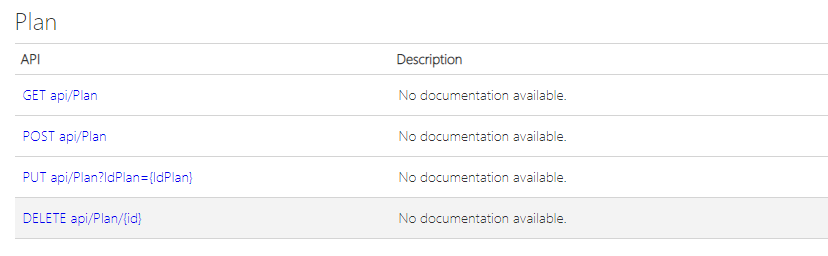
\includegraphics[width=15cm]{./Imagenes/plan}
             \end{center}
Copiamos el formato de la cadena, y luego la pegamos en Postman, donde agregaremos un nuevo plan.
 \begin{center}
			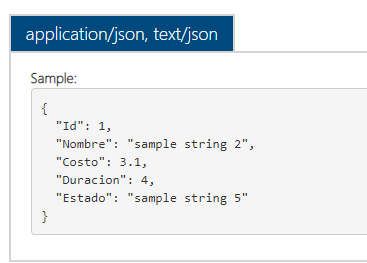
\includegraphics[width=8cm]{./Imagenes/p}
             \end{center}
 \begin{center}
			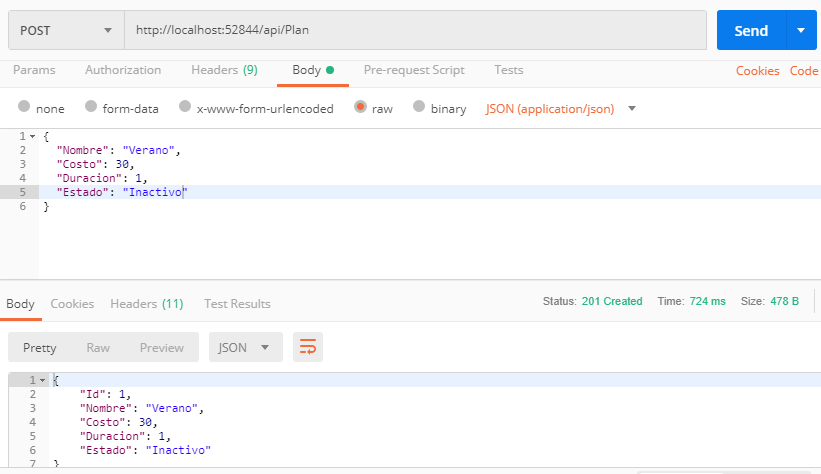
\includegraphics[width=15cm]{./Imagenes/pp}
             \end{center}
\item Del controlador Empresa, hacemos clic en POST Empresa para agregar un registro.
 \begin{center}
			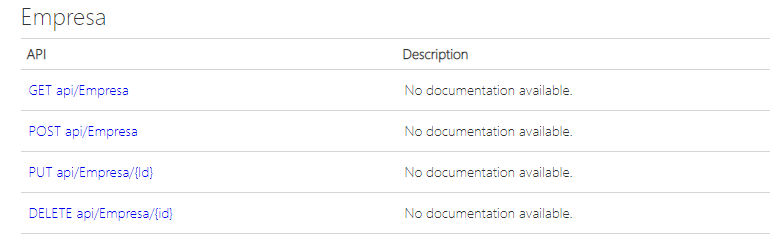
\includegraphics[width=15cm]{./Imagenes/emp}
             \end{center}
Copiamos el formato de la cadena, y luego la pegamos en Postman, donde agregaremos un nuevo empresa.
 \begin{center}
			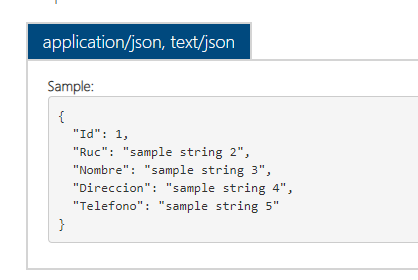
\includegraphics[width=10cm]{./Imagenes/em}
             \end{center}
 \begin{center}
			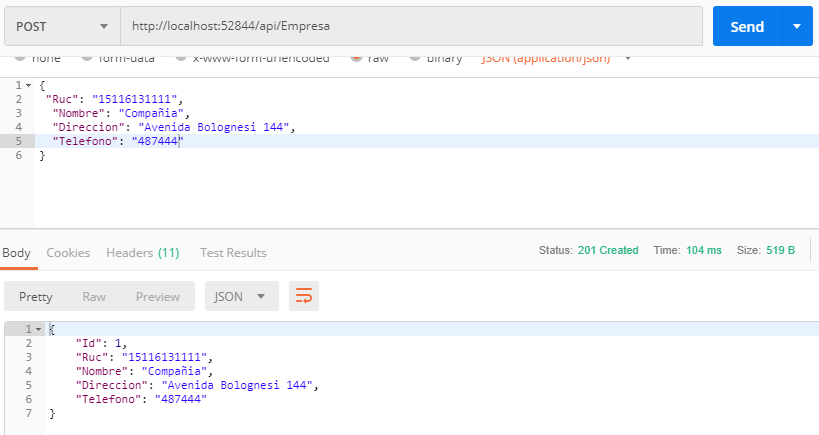
\includegraphics[width=15cm]{./Imagenes/pem}
             \end{center}

\end{itemize}



        
        
        

